\section{Free Energy}\label{sec:Free_energy}
\vspace{3cm}
\par


The free energy is a highly desirable quantity to compute. It is in essence the factor that determines how a process will proceed and the probability that a system will adopt a given state. The ability to calculate free energies from molecular simulations not only allows one to understand the underlying processes on an atomic level but also to probe states of a system not accessible experimentally. In particular, if precise and accurate estimates of the free energy of a system could be obtained directly from numerical simulations, the need to measure thermodynamic properties of a system, such as ligand-binding constants \cite{free_energy}, by experiment would be greatly reduced. This is why, for example, free energy calculations have attracted much interest in areas such as rational drug design and material science. 
Free energy calculations can be classified into two categories. The calculation of conformational free energies aims at evaluating the relative free energies of relevant conformational states of a given molecular system. The calculation of alchemical free energies on the other hand aims at evaluating the relative free energies of different molecules, which is the main objective of this work. 

Free energy is an extensive property, meaning that its magnitude depends on the amount of a substance in a given thermodynamic state, and it's expressed in two forms depending on the conditions that it is determined: The relative (Helmholtz) free energy $F$ is obtained under isochoric-isothermic conditions (NVT), whereas the relative (Gibbs) free enthalpy $G$ is obtained under isobaric-isothermic conditions (NPT). Both expressions are given by: 
\begin{equation}
    F=U-TS
    \label{eq:Helmholtz}
\end{equation}
\begin{equation}
    \begin{split}
    G&=U+PV-TS\\ 
     G&=H-TS
    \end{split}
    \label{eq:Gibbs}
\end{equation}

From an MD trajectory, described in Section \ref{sec:MD}, the statistical equilibrium averages can be obtained for any desired property of the molecular system for which a value can be computed at each point of the trajectory. Examples of such properties are the potential or kinetic energy of relevant parts of the system, structural properties and fluctuations, electric fields, diffusion constants, etc. A number of thermodynamic properties can be derived from such averages. However, two important thermodynamic quantities, the entropy and the (Gibbs or Helmholtz) free energy, generally cannot be derived from a statistical average. They are global properties that depend on the extent of phase (or configuration) space accessible to the molecular system \cite{van1988role}. Fortunately, with statistical mechanics methods one can evaluate the \textit{relative} free energy differences.


\subsection{Thermodynamic Integration}\label{subsec:TI}

The aim of thermodynamic integration is to compute the difference in a thermodynamic property (usually the free energy) of the system between some reference state and the state of interest. It make use of the fact that the free energy changes related to small perturbations of a molecular system can be determined during a simulation. Taking that fact into account, the free energy difference between two states A and B of a system can be determined from an MD simulation in which the potential energy function $V(q)$ is slowly changed such that the system slowly changes from state A to state B over a reversible path.

Since the absolute value for free energy of solvation is difficult to calculate directly, we use the fact that the free energy is a \textbf{state function}. From the thermodynamic cycle presented in Figure \ref{fig:TI_cicle} it follows that:
\begin{figure}[h]
    \centering
    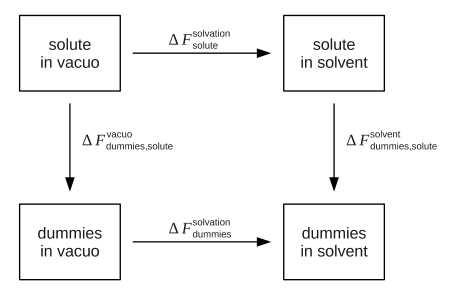
\includegraphics[scale=0.6]{Figures/Chapter 3/Ciclo_termodinamico.png}
    \caption{Thermodynamic cycle for the determination of solvation free energies}
    \label{fig:TI_cicle}
\end{figure}

\begin{equation}
    \Delta F_{solute}^{solvation} = \Delta F_{dummies,solute}^{vacuo} + \Delta F_{dummies}^{solvation} - \Delta F_{dummies,solute}^{solvent} 
\end{equation}  
The solvation free energy $\Delta F_{solute}^{solvation}$ is the work required to transfer a molecule from the gas phase into solute solution. $\Delta F_{dummies,solute}^{vacuo}$ is the work required to remove all the internal nonbonded interactions in the solute in vacuo, which is achieved by gradually mutating all atoms in a solute molecule into dummy atoms. A dummy atom is an atom for which the nonbonded interactions, i.e. Lennard-Jones and electrostatic interactions, with all other atoms are set to zero while the bonded interactions within the molecule and the masses of individual atoms are kept unchanged. $\Delta F_{dummies}^{solvation}$ is the work required to transfer the dummy solute molecule from
vacuum to the solvated phase. As the dummy molecule does not interact with the rest of the system this
term is also equal to zero. In order to determine the solvation free energy of any peptide with this method, only the free energy $\Delta F_{dummies,solute}^{solvent}$ must therefore be calculated. Since $\Delta F_{dummies,solute}^{solvent}$ is the work required to remove the solute-solvent and solute-intermolecular interactions. for this particular case, as we are interesting only in the solute-solvent interaction (Van der Waals) the intermolecular forces between the peptide atoms remain constant. 

This transition, from a particular atom to a dummy particle, works as follows:
\textbf{(1)} The Hamiltonian $H(p,q)$ is made a function of a coupling parameter $\lambda$, such that $H(p,q,\lambda)$ characterises the two different sates of interest, normal and dummy particle. 
\begin{equation}
    H(p,q,\lambda)=\sum^N_{i=1}\frac{p_i^2}{2m_i(\lambda)}+V(q,\lambda)
    \label{eq:Ham_lambda}
\end{equation}
with
\begin{equation}
    m_i(\lambda)=(1-\lambda)m_i^A +\lambda m_i^B
\end{equation}
and
\begin{equation}
    \begin{split}
        V(q,\lambda) &= \sum_{bonds,b} V(b,\lambda) + \sum_{angles,\theta} V(\theta,\lambda) + \sum_{torsion,\xi} V(\xi,\lambda)  + \\
        &   + \sum_{dihedrals,\xi} V(\psi,\lambda) + \sum_{nonb (i,j)} V(r_{ij},\lambda)
    \end{split}
    \label{eq:V_lambda}
\end{equation}

Equation \ref{eq:V_lambda} represents each one of the potential energy terms described in Equations \ref{eq:bond_inter} and \ref{eq:nonb_inter} with the couple parameter $\lambda$.
In this work, only the non bonded interaction will be modify with the coupling parameter and study the transition between the twp states. The mathematical formulation will be presented in following sections. 

\subsubsection{Gibbs Free Energy}

The Gibbs free energy of the system becomes a function of $\lambda$ and is given by: 
\begin{equation}
    G(\lambda)=-kT\ln{\Delta \lambda}
    \label{eq:DG_general}
\end{equation}
where $k$ denotes Boltzmann's cosntant, $T$ is the temperature of the system and $\Delta \lambda$ is the isobaric partition function given by: 
\begin{equation}
    \Delta \lambda= \frac{1}{h^{3N}N!}\int\int\int\exp{[(-H(p,q,\lambda)+PV)/kT]}dVdpdq
    \label{eq:part_func}
\end{equation}
where $P$ and $V$ are the pressure and the volume of the system respectively, $p$ and $q$ are the momentum and Cartesian coordinates of the N atoms. 

The free energy difference $\Delta G_{BA}$ is givne by: 
\begin{equation}
    \Delta G_{BA}= G(\lambda_B) - G(\lambda_A) = -kT\ln{\left ( \frac{\Delta \lambda_B}{\Delta \lambda_A} \right )}
\end{equation}
which can be expressed as an ensemble average by:
\begin{equation}
    \begin{split}
       &\Delta G_{BA} =-kT\ln\\\\
       &{\left \{ \frac{\int\int\int\exp{[(-H(p,q,\lambda_B)-H(p,q,\lambda_A))/kT]}\exp{[(-H(p,q,\lambda_A)+PV)/kT]}dVdpdq} {\int\int\int\exp{[(-H(p,q,\lambda_A)+PV)/kT]}dVdpdq} \right \}}\\\\
       &=-kT\ln{\left \{  \left \langle \exp{[(-H(p,q,\lambda_B)-H(p,q,\lambda_A))/kT]} \right \rangle \right \}}
    \end{split}
\label{eq:pertur}
\end{equation}
where the $\left \langle ... \right \rangle_\lambda$ mean an ensemble average over the volume $V$, the coordinates $q$ and momentum $p$ at the value $\lambda$. Equation \ref{eq:pertur} is called the perturbation formula, since only yield accurate results when state B is close to state A. If this difference is large, that change from A to B must be split up into a number of steps between intermediate states that are close enough to allow the use of Equation \ref{eq:pertur} \cite{van1988role}. Meeting this condition, $\Delta G_{BA}$ is just the sum of the individual $\Delta G$ for all intermediate steps. The differentiation of Equation \ref{eq:DG_general} with respecto to $\lambda$ at constant temperature and pressure yields:
\begin{equation}
    \begin{split}
        &\left ( \frac{\partial G(\lambda)}{\partial \lambda} \right )_{T,P}=-\left ( \frac{kT}{\Delta (\lambda)} \right ) \left [ \frac{\partial \Delta (\lambda)}{\partial \lambda} \right ]_{T,P} \\\\
        &=\frac{\int\int\int[\partial H(p,q,\lambda)/\partial \lambda] \exp{[-(Hp,q,\lambda)+PV)/kT] dV dp dq}}{\int\int\int\exp{[-(H(p,q,\lambda)+PV)/kT]dV dp dq}}\\\\
        &=\left \langle \frac{\partial H(p,q,\lambda)}{\partial \lambda} \right \rangle_\lambda
    \end{split}
\end{equation}
The free-energy difference ($\Delta G$) between two states, A and B, can be readily calculated using the TI formula:
\begin{equation}
    \Delta G_{BA}=G(\lambda_{B})-G(\lambda_{A})=\int_{\lambda =0}^{\lambda =1}\left \langle \frac{\partial H(\lambda )}{\partial \lambda } \right \rangle_\lambda d\lambda
    \label{eq:TI}
\end{equation}
 where $H(\lambda)$ is a combined potential energy function connecting the potential energy functions with a coupling parameter $\lambda$ between states $A (H_{A}; \lambda =0) $ and state $B (H_{B}; \lambda =1)$. In this methodology, state A is represent the peptide with the normal peptide-solvent interactions, while state B refers to a non-interacting dummy particle described in the previous paragraph. In the practice, the result of Equation \ref{eq:TI} is computed a every $\lambda$ point and then numerically integrated to obtain the free energy difference between the two states. Figure \ref{fig:GA_to_GB} represent this idea. 
 \begin{figure}[h]
     \centering
     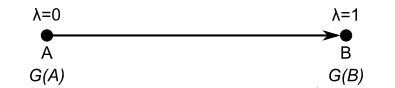
\includegraphics[scale=0.5]{Figures/Chapter 3/GA_to_GB.png}
     \caption{Transition between the states A and B with according to coupling parameter $\lambda$}
     \label{fig:GA_to_GB}
 \end{figure}
 
If $\lambda$ is being changed very slowly from $\lambda_A$ to $\lambda_B$ during a MD simulation, the integration of Equation \ref{eq:TI} can be carried out in the course of the MD run. In this way $\Delta G_{BA}$ can be obtained for rather different states A and B, as long as the continuous change in $\lambda$ is so slow that the system remains essentially in equilibrium for each intermediate value of $\lambda$.

\subsubsection{Soft-Core Potential Energy}\label{subsubsec:softcore}

A practical problem affect the predicted free energy difference and that is the presence of a \textit{"singularity"} in the function for which an ensemble average is to be determined, in this case, the Hamiltonian. When the ensemble average is obtained by MD simulation such singularities may also lead to numerical instabilities in the integration of the equations of motion \cite{beutler1994avoiding}. In general, a singularity problem arises in simulations when an observable, for which the ensemble average is to be calculated, contains regions high-energy regions of the Hamiltonian. Depending on the pathway chosen, the ensemble average of this observable may diverge. The van der Waals interaction and the electrostatic interaction between charges of equal sign (repulsive forces) become infinitely large for $r_{ij}$ approaching zero.  

In the practice, the singularity problem is often encountered when non-bonded interactions sites are to be removed, added or modify. A soft-core potential energy function is employed by GROMOS software to avoid singularities near the end-states of the TI simulations. The Lennard-Jones potential (LJ) energy function, Equation \ref{eq:gromos_LJ}, between atoms $i$ and $j$ at a state $X$ is then defined as:
\begin{equation}
    H^{VdW}_{i,j,\lambda} = \left [ \frac{C_{12}^{X}(i,j)}{\alpha_{LJ}\lambda^{2}C_{12,6}^{X}(i,j)+(r_{ji})^{6}} - C_{6}(i,j)\right ]\cdot \frac{1}{\alpha_{LJ}\lambda^{2}C_{12,6}^{X}(i,j)+(r_{ji})^{6}}
\end{equation}

The singularity at $r_{ij}=0$ is removed and the interaction function is smoothened for $\lambda=0$ and $\alpha_{LJ}$ is the softness parameter for the LJ interaction. A similar transformation is used to couple the $\lambda$ parameter to electrostatic potential (Equation \ref{eq:electrostatic}) and it's given by: 
\begin{equation}
    H^{elec}_{i,j,\lambda}=\frac{q^X_i q^X_j}{4\pi \epsilon_0 \epsilon_1}\left [ \frac{1}{\left [ \alpha_{CRF}(i,j)\lambda^2+r_{ij}^2\right ]^{\frac{1}{2}}} - \frac{\frac{1}{2}C_{rf}r{ij}^2}{\left [\alpha_{CRF}(i,j)\lambda^2+R_{rf}^2 \right ]^\frac{3}{2}} - \frac{\left ( 1-\frac{1}{2}C_{rf}\right )}{R_{rf}}\right ]
    \label{eq:softcorepot}
\end{equation}
where $q_i^X$ is the partial charge of atom $i$ and $C_{rf}$ and $R_{rf}$ are parameters of the reaction-field method \cite{tironi1995generalized}. $\alpha_{CRF}$ is the softness parameter for the electrostatic interactions, similar to $\alpha_{LJ}$ described before. Finally, the non-bonded potential energy for particles $i$, $j$ in a given state (from A to B)is calculated as:
\begin{equation}
    H_{i,j,\lambda}^{NB}= H^{VdW}_{i,j,\lambda}+H^{elec}_{i,j,\lambda}
\end{equation}
The combined non-bonded potential energy function connecting states A and B is now:
\begin{equation}
    H(r_{ij};\lambda)=\lambda H^{NB}(r_{ij};B;(1-\lambda))+(1-\lambda)H^{NB}(r_{ij};A;\lambda)
\end{equation}

Because the focus of the present study is on calculating non-polar contributions to the solvation process, the alanine molecules were treated as neutral without any partial charges on the atoms for simplicity and to avoid any electrostatic contributions to solvation. This was accomplished by set to 0 all the atomic charges of every atom in the \textbf{*.top} file. 
